\documentclass[11pt]{article}

\usepackage[margin=1in]{geometry}
\usepackage{amsmath,amssymb,amsthm}
\usepackage{tikz}
\usepackage{booktabs}
\usepackage{hyperref}
\usepackage{algorithm}
\usepackage{algpseudocode}
\usetikzlibrary{arrows.meta,positioning,fit,backgrounds}

\newtheorem{proposition}{Proposition}
\newtheorem{assumption}{Assumption}
\newtheorem{remark}{Remark}

\title{The \texttt{impjax\_toymodels} Wrapper:\\
Reduced-Coordinate Sampling of IMP Systems with BlackJAX}
\author{Design document --- \texttt{doc/design.tex}}
\date{Draft, 2026-08-13}

\begin{document}
\maketitle

\begin{abstract}
This document specifies, in full mathematical detail, how \texttt{wrapper\_impjax.py}
turns a built IMP/PMI system into a BlackJAX-samplable posterior and back again.
It fixes: (1) the reduced coordinate system used for sampling (rigid-body
quaternion/translation pairs plus flexible-bead coordinates), (2) the exact
map between that reduced state and the flat per-particle array IMP's JAX
export expects, (3) SO(3)-compliant, detailed-balance-preserving proposal
kernels for rotations, translations, and bead moves, (4) how these plug into
the existing BlackJAX RMH/SMC wrappers in this repo without reimplementing
any sampler, and (5) a GPU-aware I/O design for stat files and RMF3
trajectories. Every claim about IMP's runtime behavior below (Section
\ref{sec:bridge}) was verified empirically against the \texttt{imp} conda
environment, not assumed from documentation, since the JAX export layer in
IMP is not otherwise documented.
\end{abstract}

\tableofcontents

\section{Scope and non-negotiables}
\label{sec:scope}

Per \texttt{planning.md}, this repo must never reimplement a sampler: BlackJAX
supplies the RMH/SMC/HMC kernels (already wrapped in \texttt{rmh\_sampler.py}
and \texttt{smc\_base\_sampler.py}); this repo's only job is to supply BlackJAX
with a JIT-able log-density function and a smart, SO(3)-correct proposal.
Concretely this document designs five small, single-purpose modules:

\begin{center}
\begin{tabular}{@{}l p{9.5cm}@{}}
\toprule
Module & Responsibility \\
\midrule
\texttt{dof\_layout.py} & Index bookkeeping: which particles are sampled, in what order, as what shape. \\
\texttt{state\_sync.py} & IMP $\to$ reduced state (extract), reduced state $\to$ full IMP-shaped array (expand), reduced state $\to$ IMP (apply). \\
\texttt{proposals.py} & SO(3) rotation, translation, and bead proposal kernels; composite proposal builder. \\
\texttt{wrapper\_impjax.py} & Orchestration: build $\log\pi$, build proposal, call into \texttt{rmh\_sampler.py}, sync results back. \\
\texttt{gpu\_io.py} & Device-resident buffering, batched host flush, stat file + RMF3 writing. \\
\bottomrule
\end{tabular}
\end{center}

None of these exceed the repo's 200--300 line budget individually.

\section{System state and notation}
\label{sec:state}

A built IMP system (\texttt{BuiltSystem} in \texttt{system\_info.py}) exposes,
via \texttt{rigid\_bodies\_and\_beads()}, an ordered list of $K$ rigid bodies
and $M$ flexible (non-rigid) beads. We fix this ordering once at wrapper
construction time and never re-derive it mid-run, since every array in this
design is positional.

\paragraph{Rigid body $k$.} State is a pose
\[
  \theta_k = (q_k, t_k) \in \mathbb{S}^3 \times \mathbb{R}^3, \qquad \|q_k\| = 1,
\]
a unit quaternion $q_k = (w_k, x_k, y_k, z_k)$ (double-covering a rotation
$R(q_k) \in SO(3)$) and a translation $t_k$ of the rigid body's reference
frame. Each rigid body owns an ordered set of \emph{member} particles
$\mathcal{M}_k = \{1, \dots, n_k\}$ whose \emph{local} (internal, frame-relative)
coordinates $\ell_{k,i} \in \mathbb{R}^3$ are fixed for the lifetime of the run
(IMP: \texttt{RigidMember.get\_internal\_coordinates()}). A member's global
position is
\begin{equation}
  \label{eq:rigid-transform}
  g_{k,i}(\theta_k) = R(q_k)\, \ell_{k,i} + t_k .
\end{equation}

\paragraph{Flexible bead $m$.} State is simply its global coordinate
$x_m \in \mathbb{R}^3$.

\paragraph{Reduced state.} The full sampled state is the pytree
\[
  \theta = \big(\{q_k, t_k\}_{k=1}^K,\ \{x_m\}_{m=1}^M\big),
\]
with dimension $7K + 3M$ (4 for each quaternion, 3 for each translation, 3
per bead). BlackJAX's samplers accept an arbitrary JAX pytree as the chain
position (verified against \texttt{blackjax.mcmc.random\_walk}, which types
its position as \texttt{ArrayLikeTree} throughout), so the wrapper drives
the walk directly on the structured dict
$\theta = \{\text{quaternions}: (K,4),\ \text{translations}: (K,3),\ \text{bead\_coords}: (M,3)\}$
with no flattening required. \texttt{dof\_layout.py} additionally defines a
bijection $\mathrm{flatten}: \theta \mapsto \mathbb{R}^{7K+3M}$ (and its
inverse) used only for compact storage -- the GPU IO buffer
(Section~\ref{sec:io}) and stat-file rows -- not to satisfy any BlackJAX
requirement.

\section{The IMP $\leftrightarrow$ JAX bridge}
\label{sec:bridge}

IMP exposes, on any \texttt{IMP.core.RestraintsScoringFunction}, a private
method \texttt{\_get\_jax()} returning an object \texttt{ji} with two members:

\begin{itemize}
  \item \texttt{ji.get\_jax\_model() -> \{"xyz": ndarray(N,3), "r": ndarray(N,)\}} --
    \textbf{every} particle currently registered in the IMP \texttt{Model}
    (not just leaves: $N=531$ for a 52-leaf, 2-domain toy dimer used in
    testing), indexed by \emph{IMP particle index}. \texttt{r} is a static
    per-particle radius.
  \item \texttt{ji.score\_func(model\_dict) -> scalar} -- a pure, JAX-traceable
    function of the passed-in dict. Its value matches
    \texttt{RestraintsScoringFunction.evaluate(False)} on the corresponding
    IMP state exactly.
\end{itemize}

\begin{assumption}[Verified empirically, not documented by IMP]
\label{ass:bridge}
Three properties were confirmed by direct experiment (moving a particle and
comparing \texttt{score\_func} outputs; see repo history for the probe
scripts) and are relied on throughout this design:
\begin{enumerate}
  \item \texttt{get\_jax\_model()["xyz"]} is a \emph{live view} aliased to IMP's
    internal storage -- mutating the IMP model changes previously-fetched
    dicts too. \textbf{Every module below explicitly copies this array}
    before treating it as an immutable JAX value.
  \item \texttt{score\_func} depends \emph{only} on its argument, not on
    hidden IMP state -- passing a hand-built \texttt{\{"xyz": ..., "r": ...\}}
    with the same shape reproduces IMP's own energy for that configuration.
    This is what makes the wrapper's log-density JIT-/grad-able.
  \item Row $i$ of \texttt{"xyz"} corresponds to IMP particle index $i$
    (0-based; the integer cast of a particle's \texttt{ParticleIndex}),
    not to leaf order or selection order.
\end{enumerate}
\end{assumption}

\begin{assumption}[Rigid-body transform convention]
\label{ass:quat}
\texttt{IMP.algebra.Rotation3D(w,x,y,z)} implements the standard active
rotation
\[
  R(q)v = v + 2\big(w\,(q_v \times v) + q_v \times (q_v \times v)\big), \qquad
  q_v = (x,y,z),
\]
and \texttt{RigidBody.get\_reference\_frame().get\_transformation\_to()}
yields $(R(q_k), t_k)$ such that a member's global coordinate equals
Eq.~\eqref{eq:rigid-transform} exactly. Verified numerically to full float
precision with a synthetic single-member rigid body and a $90^\circ$
rotation.
\end{assumption}

\begin{assumption}[Auxiliary, non-sampled rows]
\label{ass:aux}
Only $52$ of $531$ rows in the toy dimer correspond to sampled leaves
(rigid-body members or flexible beads); the remainder are IMP bookkeeping
particles (hierarchy/state/molecule/residue decorators) with no bearing on
the restraints currently attached in this repo's tests. These rows are
frozen at their build-time template value for the lifetime of a sampling
run. \textbf{This is a scoped assumption, not a general guarantee}: if a
restraint is later added that reads a coarser-resolution representation not
covered by the sampled leaves, that restraint's contribution would silently
use stale coordinates. Section~\ref{sec:limitations} lists the regression
test that guards this invariant for the restraints in use today, and flags
it for re-verification whenever new restraint types are added.
\end{assumption}

\section{The expansion map $\Phi$}
\label{sec:expansion}

\texttt{state\_sync.py} builds $\Phi: \theta \mapsto \mathrm{xyz} \in \mathbb{R}^{N\times 3}$:

\begin{equation}
  \label{eq:expansion}
  \Phi(\theta)_j =
  \begin{cases}
    R(q_k)\,\ell_{k,i} + t_k & j \text{ is member } i \text{ of rigid body } k, \\
    x_m & j \text{ is flexible bead } m, \\
    \mathrm{xyz}^{\text{template}}_j & \text{otherwise (Assumption~\ref{ass:aux})}.
  \end{cases}
\end{equation}

$\mathrm{xyz}^{\text{template}}$ and $r$ are captured \emph{once}, as plain
(copied) \texttt{numpy} arrays, when the wrapper is constructed --- this is
the one and only place IMP's live-view aliasing (Assumption~\ref{ass:bridge}.1)
is touched; everything downstream is ordinary immutable JAX. The member
index sets $\{(k,i,j)\}$ and local coordinates $\{\ell_{k,i}\}$ are likewise
captured once, from \texttt{RigidMember.get\_internal\_coordinates()}, and
are treated as constants of the run (not resampled).

\paragraph{Log-posterior.} IMP restraints are energies, satisfied at low
values, so the (unnormalized) log-posterior used for Metropolis accept/reject
is
\begin{equation}
  \label{eq:logpost}
  \log \pi(\theta) = -\,\texttt{score\_func}\big(\{\text{xyz}: \Phi(\theta),\ r\}\big) \;+\; \log p_0(\theta),
\end{equation}
where $p_0$ is an optional prior over the reduced state (e.g. bounding-box or
nuisance-parameter priors); it defaults to $0$ (flat/improper) for the toy
models in \texttt{test/}.

\section{Proposal kernels}
\label{sec:proposals}

All kernels below are constructed so that the Metropolis ratio needs
\textbf{no} Hastings correction term -- i.e. proposal densities are symmetric,
$q(\theta' \mid \theta) = q(\theta \mid \theta')$ -- which is why
\texttt{rmh\_sampler.py} can plug a plain \texttt{blackjax.rmh(logdensity\_fn,
proposal)} kernel (its docstring already anticipates a caller-supplied
\texttt{proposal(key, position) -> new\_position}; we are that caller).

\subsection{Translation proposals (rigid-body and bead)}

Additive isotropic Gaussian:
\begin{equation}
  t_k' = t_k + \sigma_t \,\varepsilon, \qquad x_m' = x_m + \sigma_b\,\varepsilon,
  \qquad \varepsilon \sim \mathcal{N}(0, I_3).
\end{equation}
Symmetric by construction ($\mathcal{N}(0,I_3)$ is symmetric about $0$), so
$q(t' \mid t) = q(t \mid t')$ trivially. Rigid bodies typically use a larger
$\sigma_t$ than individual beads, reflecting the different physical scales
called out in \texttt{planning.md} (10s--100s of residues per rigid body vs.
a handful per bead).

\subsection{SO(3)-compliant rotation proposal}
\label{sec:so3}

Naively perturbing quaternion components with i.i.d.\ Gaussian noise and
renormalizing is \emph{not} SO(3)-compliant: it distorts the invariant (Haar)
measure on the rotation group and biases the proposal, which is exactly what
\texttt{planning.md} rules out. Instead we perturb in the Lie algebra
$\mathfrak{so}(3) \cong \mathbb{R}^3$ and map back via the exponential:

\begin{align}
  \omega &\sim \mathcal{N}(0, \sigma_r^2 I_3) \in \mathbb{R}^3, \\
  \delta q &= \exp(\omega) = \Big(\cos\tfrac{\|\omega\|}{2},\ \sin\tfrac{\|\omega\|}{2}\,\hat\omega\Big), \qquad \hat\omega = \omega / \|\omega\|, \\
  q_k' &= \delta q \otimes q_k \quad \text{(quaternion multiplication)}, \label{eq:qcompose}
\end{align}
with $\delta q$ taken to be the identity $(1,0,0,0)$ when $\omega = 0$ (removable
singularity of the formula at $\|\omega\|=0$). Because $\delta q$ and $q_k$
are both unit quaternions, $q_k'$ is unit norm to machine precision by
construction (a defensive renormalization is still applied to absorb
floating-point drift over many steps).

\begin{proposition}[Symmetry / detailed balance of the SO(3) proposal]
\label{prop:so3-symmetric}
The proposal kernel $q(\cdot \mid q_k)$ induced by
Eq.~\eqref{eq:qcompose} is symmetric with respect to the Haar measure on
$SO(3)$: $q(q_k' \mid q_k) = q(q_k \mid q_k')$.
\end{proposition}
\begin{proof}[Proof sketch]
$\mathcal{N}(0,\sigma_r^2 I_3)$ is symmetric under $\omega \mapsto -\omega$,
and $\exp(-\omega) = \exp(\omega)^{-1} = \delta q^{-1}$ (the conjugate
quaternion), so $\delta q$ and $\delta q^{-1}$ are equally likely draws.
Left-multiplication by a fixed rotation is measure-preserving for the Haar
measure on $SO(3)$ (a standard group-invariance fact), so the map
$q_k \mapsto \delta q \otimes q_k$ pushes the (rotation-invariant) proposal
distribution over $\delta q$ into a distribution over $q_k'$ whose density
at $q_k$, having arrived from $q_k'$ via $\delta q^{-1}$, equals the density
of arriving at $q_k'$ from $q_k$ via $\delta q$ --- i.e. $q(q_k' | q_k) =
q(q_k | q_k')$. This is the same construction used for random-walk proposals
on Lie groups in the computational statistics literature (perturb in the
tangent space at the identity, transport by the group action).
\end{proof}

\begin{remark}[Double cover]
$q$ and $-q$ represent the same rotation. The scoring function only ever
sees $R(q)$ through Eq.~\eqref{eq:rigid-transform}, which is invariant to
this sign, so no special handling is required for correctness; we simply
do \emph{not} attempt to canonicalize the sign of $q_k'$, since doing so
would not change $\log\pi$.
\end{remark}

\subsection{Composite, mode-masked proposal}
\label{sec:modes}

\texttt{planning.md} requires the user to choose, at sampling time, which
degrees of freedom move: rigid rotations only, rigid translations only,
rigid rotation+translation, flexible beads only, or all of the above. This
is implemented as a single proposal function parameterized by a boolean
mode mask $(\text{rot}, \text{trans}, \text{bead}) \in \{0,1\}^3$: each
excluded component's step is replaced with the identity ($\sigma \to 0$),
which trivially preserves detailed balance (a deterministic identity map is
its own reverse). Concretely, per MH step, \texttt{proposals.py} draws
independent noise for every rigid body and bead (vectorized over $K$ and
$M$ with \texttt{jax.vmap}) and masks out the disabled groups \emph{before}
composing/adding, so the same compiled proposal function serves every mode
without retracing.

\section{Metropolis correctness}
\label{sec:mh}

For a symmetric proposal $q(\theta'|\theta) = q(\theta|\theta')$, the
Metropolis acceptance probability
\begin{equation}
  \label{eq:accept}
  \alpha(\theta \to \theta') = \min\Big(1,\ \exp\big[\log\pi(\theta') - \log\pi(\theta)\big]\Big)
\end{equation}
satisfies detailed balance $\pi(\theta)\,q(\theta'|\theta)\,\alpha(\theta\to\theta')
= \pi(\theta')\,q(\theta|\theta')\,\alpha(\theta'\to\theta)$ by the standard
Metropolis argument. Section~\ref{sec:so3} establishes symmetry for the
rotation component; translation and bead components are symmetric Gaussian
steps; the masked/identity components are trivially symmetric. The product
proposal over independent rigid bodies and beads is therefore symmetric as a
whole, so Eq.~\eqref{eq:accept} applies directly with \emph{no} Hastings
ratio term -- matching the \texttt{blackjax.rmh(logdensity\_fn, proposal)}
contract already documented in \texttt{rmh\_sampler.py}.

\section{Wrapper pipeline}
\label{sec:pipeline}

\begin{figure}[h]
\centering
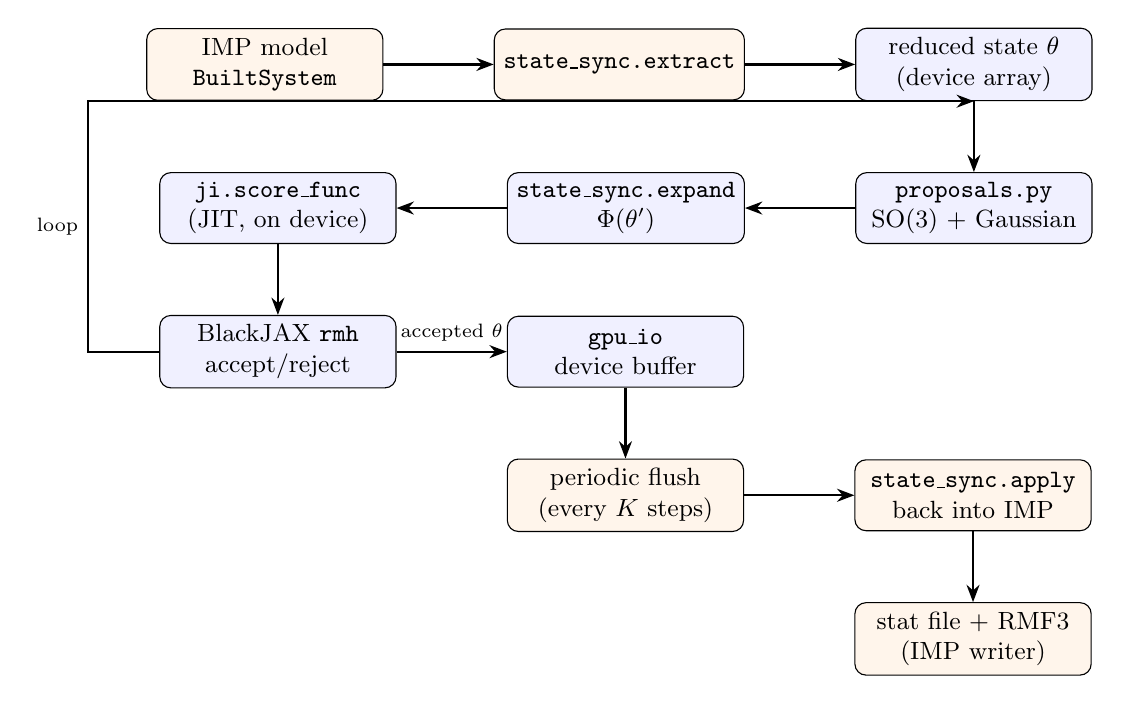
\begin{tikzpicture}[
  node distance=9mm and 14mm,
  box/.style={draw, rounded corners, align=center, minimum height=9mm, minimum width=30mm, font=\small},
  gpu/.style={box, fill=blue!6},
  cpu/.style={box, fill=orange!8},
  arr/.style={-{Stealth[length=2.2mm]}, thick}
]
  \node[cpu] (imp) {IMP model \\ \texttt{BuiltSystem}};
  \node[cpu, right=of imp] (extract) {\texttt{state\_sync.extract}};
  \node[gpu, right=of extract] (theta) {reduced state $\theta$ \\ (device array)};
  \node[gpu, below=of theta] (prop) {\texttt{proposals.py} \\ SO(3) + Gaussian};
  \node[gpu, left=of prop] (expand) {\texttt{state\_sync.expand} \\ $\Phi(\theta')$};
  \node[gpu, left=of expand] (score) {\texttt{ji.score\_func} \\ (JIT, on device)};
  \node[gpu, below=of score] (mh) {BlackJAX \texttt{rmh} \\ accept/reject};
  \node[gpu, right=of mh] (buf) {\texttt{gpu\_io} \\ device buffer};
  \node[cpu, below=of buf] (flush) {periodic flush \\ (every $K$ steps)};
  \node[cpu, right=of flush] (apply) {\texttt{state\_sync.apply} \\ back into IMP};
  \node[cpu, below=of apply] (out) {stat file + RMF3 \\ (IMP writer)};

  \draw[arr] (imp) -- (extract);
  \draw[arr] (extract) -- (theta);
  \draw[arr] (theta) -- (prop);
  \draw[arr] (prop) -- (expand);
  \draw[arr] (expand) -- (score);
  \draw[arr] (score) -- (mh);
  \draw[arr] (mh) -- node[above,font=\scriptsize]{accepted $\theta$} (buf);
  \draw[arr] (mh.west) -- ++(-0.9,0) |- (theta.south) node[pos=0.25,left,font=\scriptsize]{loop};
  \draw[arr] (buf) -- (flush);
  \draw[arr] (flush) -- (apply);
  \draw[arr] (apply) -- (out);
\end{tikzpicture}
\caption{Wrapper data flow. Blue boxes stay resident on device across many
MCMC steps (no host round-trip); orange boxes are host/CPU-side and IMP-aware.
The MH loop only touches the host every $K$ steps, at the \texttt{gpu\_io}
flush boundary (Section~\ref{sec:io}).}
\label{fig:pipeline}
\end{figure}

\begin{algorithm}[h]
\caption{\texttt{wrapper\_impjax.run\_sampling} (single-mode RMH; SMC-tempered variant reuses the same $\log\pi$/proposal and calls \texttt{smc\_base\_sampler.py} instead)}
\begin{algorithmic}[1]
\State $\texttt{built} \gets$ \texttt{BuiltSystem} (already constructed by the user's setup script)
\State $\texttt{ji} \gets \texttt{sf.\_get\_jax()}$; $\ \texttt{layout} \gets \texttt{dof\_layout.build(built)}$
\State $\texttt{template}, r \gets$ copy of $\texttt{ji.get\_jax\_model()}$ \Comment{one-time, breaks aliasing (Assumption \ref{ass:bridge}.1)}
\State $\theta_0 \gets \texttt{state\_sync.extract(built, layout)}$
\State $\log\pi(\theta) \gets -\texttt{ji.score\_func}(\{\text{xyz}: \texttt{state\_sync.expand}(\theta, \texttt{layout}, \texttt{template}),\, r\})$
\State $\texttt{proposal} \gets \texttt{proposals.build\_composite}(\texttt{layout}, \sigma_r, \sigma_t, \sigma_b, \texttt{mode})$
\State run \texttt{rmh\_sampler.run\_rmh\_sampling}$(\log\pi, \theta_0, \texttt{proposal}, \dots)$ \Comment{unmodified existing sampler code}
\State every $K$ accepted steps: \texttt{gpu\_io.flush} $\to$ \texttt{state\_sync.apply} $\to$ write stat row + RMF3 frame
\end{algorithmic}
\end{algorithm}

\section{GPU-aware I/O}
\label{sec:io}

Two competing constraints: RMF3 writing is IMP-native and CPU-only (no GPU
path exists or is being built --- \texttt{planning.md} explicitly forbids
reimplementing infrastructure that already works), while constant
device$\to$host synchronization to write every step would dominate runtime on
GPU. The design:

\begin{enumerate}
  \item Run $K$ MCMC steps entirely on-device inside a single
    \texttt{jax.lax.scan}, accumulating $\theta_t$ (or just accepted-state
    deltas) into a device-resident buffer of shape $(K, 7K{+}3M)$.
  \item Call \texttt{jax.block\_until\_ready} once per block and transfer the
    whole buffer to host in one copy (batched, not per-step) --- this is the
    same batching discipline already used for scoring in
    \texttt{smc\_base\_sampler.batched\_vmap}.
  \item On the host, replay each flushed $\theta_t$ through
    \texttt{state\_sync.apply} (writes rigid-body reference frames and bead
    coordinates back into the live IMP model) and append one row to the stat
    file and one frame to the open RMF3 handle.
  \item The RMF3/stat writer stays open across the whole run (one file
    handle, incremental frame writes) rather than reopening per block.
\end{enumerate}

$K$ (the flush interval) is a tunable knob trading host-transfer overhead
against peak device memory for the buffer -- exactly the same
batch-size trade-off already exposed as \texttt{score\_batch\_size} in
\texttt{smc\_base\_sampler.py}, so \texttt{gpu\_io.py} reuses that naming
convention for consistency.

\emph{Status (added 2026-08-14):} step 1 above (true on-device
\texttt{jax.lax.scan} accumulation across a block before a single host
transfer) is not yet implemented in \texttt{custom\_rmh.py} or
\texttt{smc\_fixed\_schedule.py} -- both currently pull every saved sample
to host individually inside a Python loop, then flush the whole
already-host-side list through \texttt{gpu\_io.write\_block} in one batched
pass at the end of the run (steps 3-4 above, which \emph{are} implemented).
This is a tracked follow-up, not a design change.

\section{Fixed-schedule SMC}
\label{sec:smc}

A second sampler sits alongside the RMH path of Section~\ref{sec:pipeline}:
Sequential Monte Carlo with a \emph{fixed}, user-specified temperature
ladder and \emph{no} adaptive tuning of step sizes or schedule spacing --
the ``base'' SMC sampler, as opposed to a tuned/adaptive-tempered variant
(reserved for a future, separate file, \texttt{smc\_adaptive\_tempered.py};
the two must never share a file so one can be swapped or deleted without
touching the other). Implemented in \texttt{smc\_fixed\_schedule.py}, driven
from the wrapper via \texttt{wrapper\_impjax.run\_smc\_sampling}.

\subsection{Particle population and tempered target}

SMC maintains a population of $N$ independent copies of the reduced state,
$\{\theta^{(1)}, \dots, \theta^{(N)}\}$, each an ordinary
$\theta = (\{q_k,t_k\}, \{x_m\})$ from Section~\ref{sec:state}, batched as a
pytree with a leading $N$ axis on every leaf. The target at temperature
$\lambda \in [0,1]$ is
\[
  \pi_\lambda(\theta) \;\propto\; p_0(\theta)\, L(\theta)^\lambda, \qquad
  \log \pi_\lambda(\theta) = \log p_0(\theta) + \lambda \log L(\theta),
\]
where $L(\theta) = \exp(-\texttt{score\_func}(\Phi(\theta)))$ is the bare
IMP-derived likelihood term (Eq.~\eqref{eq:logpost} without any prior mixed
in) and $p_0$ is the same optional prior as Eq.~\eqref{eq:logpost}. Because
\texttt{build\_log\_prob}'s \texttt{log\_prob\_fn} already folds the prior
in, \texttt{wrapper\_impjax.py} exposes a separate
\texttt{log\_likelihood\_fn} (bare $\log L$) for this tempering split, so a
supplied prior is not double-counted between the $\lambda=0$ term and the
$\lambda$-weighted likelihood term.

\subsection{Initial population}

With no informative prior sampler available (the toy models here default to
$p_0 \equiv 1$), the initial population is built by replicating the
current IMP-extracted state $N$ times and applying one independent draw of
the SO(3)-aware proposal (Section~\ref{sec:proposals}) to each copy, so the
population starts spread out rather than identical:
\[
  \theta^{(i)}_0 = \texttt{proposal}(\text{key}_i,\ \theta_{\text{IMP}}), \qquad i = 1,\dots,N.
\]

\subsection{Algorithm}

Standard SMC (Del Moral et al., 2006), reusing
\texttt{smc\_base\_sampler.py}'s schedule functions
(\texttt{SCHEDULE\_REGISTRY}: linear/geometric/sigmoid, generic over array
shape, imported directly, not reimplemented) and \texttt{blackjax.smc.base}
for the actual reweight/resample/mutate step -- no SMC algorithm is
reimplemented. At each step $t$ (schedule value $\lambda_t$):
\begin{enumerate}
  \item \textbf{Reweight:} $w_t(\theta) = (\lambda_t - \lambda_{t-1})\log L(\theta)$.
  \item \textbf{Resample:} systematic resampling
    (\texttt{blackjax.smc.resampling.systematic}), unmodified.
  \item \textbf{Mutate:} $n_{\text{mcmc}}$ sweeps of the same symmetric
    proposal used for RMH, targeting $\pi_{\lambda_t}$, via
    \texttt{blackjax.rmh.build\_kernel()} vmapped over the $N$ particles --
    the same no-Hastings-correction argument of
    Section~\ref{sec:mh}/Proposition~\ref{prop:so3-symmetric} applies
    unchanged, since the mutation kernel is identical to
    Section~\ref{sec:proposals}'s.
\end{enumerate}
\texttt{blackjax.smc.base.init}/\texttt{step} accept an arbitrary pytree
population directly (particle count inferred from the leading dimension of
the first leaf) -- verified against the installed BlackJAX before writing
this module, not assumed -- so no flattening of $\theta$ is needed here
either, consistent with Section~\ref{sec:state}. Only
\texttt{smc\_base\_sampler.py}'s own \texttt{batched\_vmap} scoring helper
turned out \emph{not} to be reusable (it assumes a plain
$(N,\text{n\_dims})$ array); \texttt{smc\_fixed\_schedule.py} defines a
small local pytree-native equivalent rather than editing that file.

\subsection{Best-particle-only output}

Unlike RMH, where every saved sample is written out, SMC output is
deliberately pruned: at each temperature step (including the initial one)
the single best-scoring particle,
$\theta^\star_t = \arg\max_i \log\pi(\theta^{(i)}_t)$ (full, $\lambda=1$
log-posterior, for reporting), is recorded; the other $N-1$ particles at
that step are discarded. \texttt{run\_smc\_sampling} writes exactly this
sequence $\{\theta^\star_0, \dots, \theta^\star_T\}$ through
\texttt{gpu\_io.write\_block} -- one RMF3 frame per temperature step -- so
the trajectory shows the best model's progression through the anneal. This
mirrors IMP's own \texttt{IMP.pmi.macros.ReplicaExchange} with its
\texttt{number\_of\_best\_scoring\_models} set to 1, which is the natural
comparison baseline (Section~\ref{sec:comparison}).

\subsection{Untuned defaults}

\begin{center}
\begin{tabular}{@{}ll@{}}
\toprule
Parameter & Default (\texttt{smc\_fixed\_schedule.py}) \\
\midrule
$N$ (particles) & 100 \\
Temperature steps & 20 \\
Schedule & linear \\
MCMC sweeps per step & 10 \\
\bottomrule
\end{tabular}
\end{center}
These are deliberately modest, fixed values -- no adaptive selection -- so
a comparison run finishes in reasonable time; the adaptive-tempered variant
(future, separate file) is where per-run tuning belongs.

\section{DEBUG-mode score verification}
\label{sec:debug}

IMP's CPU scoring implementation is the existing, extensively tested
ground truth; the JAX export (Section~\ref{sec:bridge}) is the newer
implementation being verified against it, never the reverse. When
\texttt{debug=True} (\texttt{run\_sampling}/\texttt{run\_smc\_sampling}),
every \texttt{debug\_every} steps (RMH) or temperature steps (SMC --
typically far fewer of them, so the default is every step there) the
current $\theta$ is synced into the live IMP model
(\texttt{state\_sync.apply}) and its CPU score compared against the JAX
score already used for sampling (recovered as $-\log\pi_{\text{JAX}}$,
undoing Eq.~\eqref{eq:logpost}'s sign), via
\texttt{score\_verification.ScoreComparisonWriter}. Every checkpoint is
appended to a CSV (\texttt{step, jax\_score, imp\_score, abs\_diff}); a
mismatch above $10^{-3}$ (absolute) is logged as a warning. Checking is
throttled, not per-step, because a CPU \texttt{evaluate()} call is
comparatively expensive -- checking every step would erase the point of
sampling on JAX/GPU in the first place.

\emph{Empirical result (2026-08-14):} on the connectivity-only toy system
of Section~\ref{sec:bridge}, JAX and CPU-IMP scores agree to floating-point
precision at every checkpoint (measured $|\Delta| = 0$). On the KCOIL/ECOIL
example system, which additionally includes an excluded-volume restraint,
IMP itself emits \texttt{"No JAX support for close pairs, so using all
possible pairs; this may be slow"}, and a small but consistent absolute
mismatch appears ($\approx 137$ against scores of order $10^6$, i.e.
$\sim 0.0035\%$ relative, stable across many steps and both samplers). This
is flagged as a localized, IMP-side JAX-support gap for that specific
restraint type -- not a defect in this repository's expansion map $\Phi$ or
state-sync machinery, which is exactly what Section~\ref{sec:expansion}'s
own regression test already isolates and confirms (perturbing only
non-sampled rows does not move the score; the discrepancy tracks the
restraint type, not the sync code).

\section{Timing methodology}
\label{sec:timing}

All wall/CPU timing in this package goes through \texttt{timing.py}'s
\texttt{TimingSnapshot} (\texttt{start\_timing}/\texttt{elapsed\_timing}),
which pairs \texttt{time.perf\_counter()} (monotonic, unaffected by system
clock adjustments -- the standard choice for wall-clock benchmarking in
Python) with \texttt{time.process\_time()} (CPU time, excludes time spent
blocked/sleeping). \texttt{custom\_rmh.py} and \texttt{smc\_fixed\_schedule.py}
both report both figures at completion; the sampler-comparison example
(Section~\ref{sec:comparison}) uses the same utility around each sampler
call rather than ad hoc \texttt{time.time()}.

\section{Sampler comparison}
\label{sec:comparison}

\texttt{examples/run\_kcoil\_ecoil\_sampling.py} runs and times any
combination of three samplers on the KCOIL/ECOIL system: BlackJAX RMH
(\texttt{run\_sampling}), BlackJAX fixed-schedule SMC
(\texttt{run\_smc\_sampling}), and IMP's own native
\texttt{IMP.pmi.macros.ReplicaExchange} on an identically-scored system, as
the ground-truth-\emph{implementation} baseline (distinct from the
ground-truth-\emph{score} role IMP's CPU scorer plays in
Section~\ref{sec:debug} -- here the whole sampler, not just the score
function, is IMP's). Each selected sampler is given its own freshly built
system: sampling mutates the live IMP model in place, so reusing one system
across samplers would bias whichever ran second. A comparison table
(sampler, wall time, CPU time, final/best score) is printed and appended to
the shared run log.

\begin{assumption}[Cross-sampler start states are not bit-identical]
IMP's \texttt{shuffle\_configuration} (its own C++ RNG) and BlackJAX's
\texttt{jax.random.PRNGKey} (a separate PRNG system) cannot be seeded into
agreement; each sampler's freshly-built system is independently randomized
with the same \emph{parameters}, not the same starting coordinates.
Reported timings and final scores should be read as characteristic of each
sampler's behavior on this system, not as a controlled single-trajectory
comparison.
\end{assumption}

\emph{Empirical result (2026-08-14, toy-scale smoke test):} on a
single-copy KCOIL/ECOIL system with deliberately small step counts, IMP's
native replica exchange was faster in wall time than either BlackJAX
sampler ($0.94\mathrm{s}/100$ frames vs.\ $2.31\mathrm{s}/100$ RMH steps and
$10.70\mathrm{s}$ for a 15-particle, 6-temperature-step SMC run). This is
expected at this scale: JIT compilation overhead is not yet amortized over
enough steps, and \texttt{smc\_fixed\_schedule.py}'s per-temperature-step
retracing of \texttt{update\_fn}/\texttt{weight\_fn} (inherited from
\texttt{smc\_base\_sampler.py}'s identical pattern) adds further constant
overhead per step. Whether BlackJAX overtakes IMP's native sampler is
expected to depend on step count, system size, and GPU availability --
exactly what this comparison script exists to measure, not to assume.

\section{Module layout}
\label{sec:modules}

\begin{center}
\small
\begin{tabular}{@{}l p{5.3cm} p{3.2cm}@{}}
\toprule
File & Key functions & Depends on \\
\midrule
\texttt{dof\_layout.py} & \texttt{build}, \texttt{flatten}, \texttt{unflatten}, \texttt{mode\_mask} & \texttt{system\_info.BuiltSystem} \\
\texttt{state\_sync.py} & \texttt{extract}, \texttt{expand}, \texttt{apply} & \texttt{dof\_layout} \\
\texttt{proposals.py} & \texttt{rotation\_step}, \texttt{translation\_step}, \texttt{build\_composite} & \texttt{dof\_layout} \\
\texttt{custom\_rmh.py} & \texttt{run\_custom\_proposal\_rmh} & \texttt{blackjax.rmh}, \texttt{timing} \\
\texttt{smc\_fixed\_schedule.py} & \texttt{run\_fixed\_schedule\_smc} & \texttt{smc\_base\_sampler} (schedules only), \texttt{blackjax.smc}, \texttt{timing} \\
\texttt{score\_verification.py} & \texttt{ScoreComparisonWriter}, \texttt{make\_debug\_callback} & \texttt{state\_sync} \\
\texttt{logging\_config.py} & \texttt{configure\_logging} & stdlib \texttt{logging} only \\
\texttt{gpu\_io.py} & \texttt{TrajectoryWriter}, \texttt{write\_block} & \texttt{state\_sync} \\
\texttt{wrapper\_impjax.py} & \texttt{build\_log\_prob}, \texttt{run\_sampling}, \texttt{run\_smc\_sampling} & all of the above \\
\bottomrule
\end{tabular}
\end{center}

Each file ships with a focused \texttt{test/test\_\{module\}.py} (per the
repo's non-negotiable testing rule), runnable in the \texttt{imp} conda
environment, which is the only environment in this repo with both IMP and
BlackJAX installed together.

\section{Assumptions and limitations}
\label{sec:limitations}

\begin{itemize}
  \item Assumption~\ref{ass:aux} (frozen auxiliary rows) is scoped to the
    restraints exercised by \texttt{test/test\_imp\_system.py} and
    \texttt{test/test\_systeminfo.py} today (connectivity, excluded volume).
    A regression test asserts that perturbing a non-sampled row does not
    change \texttt{score\_func}'s output for the current restraint set; this
    test must be revisited whenever a new restraint type (e.g.\ a multi-resolution
    EM or crosslink restraint reading a coarser bead) is added.
  \item Nuisance parameters (copy number, calibration constants, etc.,
    mentioned in \texttt{planning.md}) are out of scope for this document;
    the reduced state $\theta$ and $\log p_0(\theta)$ in
    Eq.~\eqref{eq:logpost} are designed to be extended with an additional
    pytree branch for them without changing the rigid-body/bead machinery.
  \item \emph{Update, 2026-08-14:} the fixed-schedule SMC variant is no
    longer deferred -- see Section~\ref{sec:smc}. Convergence diagnostics
    (BlackJAX's built-in \texttt{effective\_sample\_size}/
    \texttt{potential\_scale\_reduction}) remain deferred to a separate,
    later, self-contained module per \texttt{planning.md}, as does the
    \emph{adaptive}-tempered SMC variant (Section~\ref{sec:smc}'s
    reserved, not-yet-written \texttt{smc\_adaptive\_tempered.py}).
  \item The excluded-volume-related JAX/CPU score mismatch reported in
    Section~\ref{sec:debug} ($\sim 0.0035\%$ relative) is unresolved and
    IMP-side (its own warning names the cause: no JAX support for close
    pairs, so it falls back to all-pairs). Re-run the debug check in
    Section~\ref{sec:debug} if IMP's JAX support for that restraint changes.
  \item \texttt{smc\_fixed\_schedule.py} redefines (and therefore retraces)
    \texttt{update\_fn}/\texttt{weight\_fn} as fresh JIT closures every
    temperature step, inherited unchanged from
    \texttt{smc\_base\_sampler.py}'s identical pattern. This is a real,
    measured performance cost at toy scale (Section~\ref{sec:comparison})
    and a candidate optimization (e.g.\ closing over $\lambda$ as a traced
    argument instead of a Python closure constant) if SMC needs to beat
    RMH/IMP-native timings on larger systems.
\end{itemize}

\end{document}
